\documentclass[letterpaper]{article}
\usepackage[utf8]{inputenc}  
\usepackage[T1]{fontenc}
\usepackage{natbib, alifexi}
\usepackage[francais]{babel}
\usepackage{datetime}
\usepackage{fancyhdr}
\usepackage{lastpage}

\title{Ordonnancement dans la famille Linux : État de l'art \\
INFO-F-308}
\author{Youri Hubaut \\
\mbox{23 mai 2016}\\
youri.hubaut@ulb.ac.be}

\begin{document}

\pagestyle{fancy}
\fancyhf{}
\renewcommand{\headrulewidth}{0pt}
\cfoot{\thepage}

\maketitle

\begin{abstract}

En tant qu'une des parties principales de la gestion des ressources, les ordonnanceurs se doivent d'être rapides et justes. Il est donc important de s'assurer de leur bon fonctionnement au travers de la preuve formelle ou des tests et d'étudier les avancées relatives à ceux-ci. Dans ce travail, nous tenterons de retracer l'évolution des ordonnanceurs de processus dans la famille Linux. Des premières versions jusqu'aux dernières avancées du noyau.

\end{abstract}

\section{Introduction}

Mais qu'est-ce que l'ordonnancement? Eswaran, Gray, Lorie et Traiger \citep{Eswaran:1976:NPC:360363.360369} tentent de définir ce concept comme étant le processus de répartition d'un ensemble de transactions entre différents acteurs. Ces transactions se décomposent en séquences d'étapes visant à accomplir divers travaux. De manière plus générale, on qualifie d'ordonnanceur tout programme visant à partager le travail entre les différentes ressources et acteurs tout en déterminant l'ordre dans lequel celles-ci seront attribuées.

Ce terme est relativement large et englobe plusieurs paradigmes. Généralement, il tend à désigner la gestion des différents processus dans des systèmes d'exploitations multitâches. On qualifie un système d'exploitation de multitâche, si celui-ci peut interlacer \og simultanément \fg ~l'exécution de plusieurs processus. Cela donne, sur des machines avec un seul processeur, l'illusion que de multiples programmes s'exécutent simultanément. Par la suite, nous considérerons que chaque processus s'occupe de la réalisation d'un ensemble de tâches par le biais d'un ou de plusieurs \textit{threads}. On utilise également la notion de préemption lorsque les processus ne choisissent pas activement de passer la main \citep{Bach:1986:DUO:8570}. À noter qu'une terminologie \citep{Casavant:1988:TSG:630789.630963} et des classifications \citep{DBLP:journals/tc/WangM85} ont été proposées afin d'y voir un peu plus clair dans cette grande famille.

Les ordonnanceurs peuvent avoir différents objectifs: maximiser la quantité de travail effectué par unité de temps, minimiser le temps de réponse (le délai qui s'écoule entre le début du travail et son exécution), minimiser la latence (le délai entre son début et sa fin), économiser la batterie ou encore maximiser l'équité (\textit{fairness}) en répartissant les ressources au mieux entre les différents acteurs tout en prenant en compte leurs caractéristiques intrinsèques.
Ils dépendent également des buts visés par l'environnement: job, interactive, ou temps réel \citep{Hansen:1973:OSP:540365}.

En outre, on demande que les ordonnanceurs soient performants et efficaces. Une gestion optimale des ressources afin de faire bénéficier au maximum les utilisateurs sans subir le surcoût associé au système d'ordonnancement lui-même. Généralement, le choix d'ordonnancement est effectué dans quatre cas: lorsqu'un programme se termine, lors d'une interruption E/S, lors d'une barrière implicite ($mutex$) ou encore lorsque le quantum de temps associé expire \citep{Bovet:2005:ULK:1077084}.

On distingue trois grandes familles: les jobs, interactifs et temps réel. Toutes tentent d'assurer une certaine équité et d'équilibrer les ressources au maximum. Les jobs se concentrent sur le traitement des calculs intensifs et visent à maximiser le nombre de travaux effectués, à réduire le délai entre le début de la tâche et sa fin tout en faisant tourner le CPU au maximum de ses capacités. Les interactifs correspondent davantage à la vision conventionnelle d'un OS; ils répondent rapidement aux demandes de l'utilisateur et essayent de contenter ses attentes au niveau des performances. Enfin, les temps réels qui visent à réaliser des objectifs dans des limites imparties et ainsi assurer une meilleure prédictabilité \citep{Tanenbaum:2005:OSD:1076555}.

\section{Les types Job}

Les ordonnanceurs de types Job, dédiés à des tâches de calculs intensifs, ont un statut un peu particulier. En effet, il existe de très nombreux algorithmes conçus spécialement pour eux \citep{journals/cce/MendezCGHF06}. Toutefois, dans le cas de Linux, l'habitude consiste à créer sa propre grille horaire au travers des logiciels hérités de Unix: \textit{Crontab} pour les tâches récurrentes et les commandes simplifiées \textit{At} pour les ponctuelles et \textit{Batch} pour démarrer le travail directement \citep{x1994x}.

Il faut signaler que Linux n'est pas un système d'exploitation spécialement conçu pour ce genre de besoins et qu'il est préférable alors d'utiliser des technologies plus adaptées comme celles des \textit{mainframes} ou des \textit{supercomputers} qui peuvent potentiellement utiliser des variantes de Linux \citep{Encyclopedia:2011}.

\section{Les types interactifs}

\subsection{Débuts}

Au début, les ordonnanceurs interactifs de Linux se limitaient au respect de la norme \textit{POSIX} qui définit: SCHED\_FIFO, SCHED\_RR, SCHED\_SPORADIC (apparu en 2008, sorte de temps réel) et SCHED\_OTHER (libre à l'implémentation) \citep{6506091}. Et plus précisément, les premières versions de Linux (1.2) semblent utiliser par défaut l'un des algorithmes les plus classiques d'ordonnancement qu'est le \textit{round robin with circular runqueue} \citep{Maxwell:1999:LCK:519502, Beck:1996:LKI:547935}. Les classes d'ordonnancements de \textit{POSIX} ne seront introduites réellement que dans le noyau 2.2 en même temps que le support du SMP \citep{ScalableLinuxScheduling}.

L'algorithme consiste à attribuer un quantum de temps fixe à chaque processus. Celui-ci peut être entièrement consommé ou non, s'il s'arrête ou se bloque. L'ordonnanceur sélectionne alors le processus suivant dans ceux étant prêts à être exécuté, chargés en mémoire et préemptés dans la file. Si aucun n'est éligible, le processeur attend jusqu'à la prochaine interruption \citep{corbato1962experimental}. Le problème est de déterminer un quantum de temps idéal afin que le \textit{context switch} ne soit pas trop pénalisant si le délai est trop court ou pas assez réactif si trop long. En outre, il répond difficilement à la notion de \textit{burst}, bonus de priorité, accordé à des processus qui ne font qu'attendre \citep{Bach:1986:DUO:8570}. Il a l'avantage d'être rapide et relativement simple à implémenter.

\subsection{$O(n)$}

Utilisé dans les versions 2.4 à 2.6 du noyau Linux, cet ordonnanceur divise le temps processeur en \og époque \fg. Dans chacune des ces époques, chaque tâche peut être exécutée jusqu'à la fin de son quantum de temps. Si elle ne l'utilise pas complètement, la moitié du temps restant est reporté pour l'époque suivante. Les processus sont sélectionnés sur base d'une métrique déterminée par l'implémentation et la priorité de chaque tâche exécutable est déterminée lors d'un changement de contexte \citep{Bovet:2005:ULK:1077084}.
Cet ordonnanceur doit donc l'origine de son nom au fait que chaque priorité associée à un processus est réévaluée lors de l'appel à l'algorithme. Il était donc peu efficace et surtout passait difficilement à l'échelle. Il éprouve des difficultés au-delà de 100 \textit{threads} actifs \citep{Nieh:2001:VRO:647055.715911}.

\subsection{$O(1)$}

Afin de régler les problèmes associés à l'ordonnanceur $O(n)$, Ingo Molnár a introduit son $O(1)$ au noyau 2.6, visant à minimiser le surcoût lié au changement de contexte. À cette époque, beaucoup de changements ont été apportés au noyau. Plusieurs travaux ont été effectués afin de modifier l'architecture du système d'ordonnancement et de certains problèmes liés au \textit{Big Kernel Lock} \citep{bryant2003linux} qui empêchaient la préemption dans certaines parties du noyau. À noter également que dans la version 2.6.16, a été rajouté SCHED\_BATCH et dans la 2.6.23, SCHED\_IDLE qui sont respectivement des politiques intensives et modérées appliquées au SCHED\_OTHER \citep{Pabla:2009:CFS:1594371.1594375}. 

L'algorithme en lui-même consistait en une série de \textit{runqueue} constituée de deux listes: l'une contenant les processus actifs et l'autre, ceux étant expirés. Chaque processus reçoit un quantum fixe de temps, déterminé par la priorité associée à ce genre de tâches, après lequel il est transféré vers l'autre liste. Lorsque la liste est vidée de tous ceux en attentes d'exécution, les pointeurs vers listes sont échangés et le travail reprend \citep{Love:2010:LKD:1855096}.

L'algorithme portera mieux son nom $O(1)$ après le noyau 2.6.8.1 qui utilisera les fameuses \textit{runqueue} de 0 à 140 et des \textit{priority arrays}. Son interactivité sera également amélioré par Con Kolivas \citep{Aas05understandingthe}.

Le problème de cet ordonnanceur est qu'il est souvent difficile de différencier les tâches interactives des non-interactives. En effet, on peut essayer d'identifier les processus interactifs en analysant leur temps moyen d'inactivité; ceux ayant un grand temps étant probablement interactifs. Il est alors possible de leur accorder un bonus de priorité, ce qui peut potentiellement déséquilibrer l'équité \citep{4631872}.

\subsection{CFS}

Enfin, dans le noyau 2.6.23, est incorporé l'implémentation, réalisée par Con Kolivas, de ce qui s'appelait le \textit{Fair-share scheduling} au doux nom de \textit{Rotating Staircase Deadline} et \textit{Staircase Process}, inspiré du \textit{Completely Fair Scheduler} de Molnár \citep{PATCHCFS}.

L'algorithme utilise un arbre rouge-noir \citep{lozi2016linux} pour répartir le temps entre les différentes tâches et stocke le temps effectué par chacun dans les \textit{sched\_entities}, qui sont héritées de \textit{task\_struct} sorte de descripteur de processus, apparu avec le patch pour le nouvel ordonanceur \citep{Pabla:2009:CFS:1594371.1594375}. Ces nœuds sont indexés par le temps d'exécution processeur en nanosecondes. Un temps maximum est également calculé pour chacun des processus et qui est déterminé comme étant celui correspondant à la répartition la plus équitable entre tous les processus. Ce temps est défini comme étant égal au temps attendu avant d'être exécuté divisé par le nombre de processus. En effet, s'il y a $N$ processus, chacun devrait obtenir un $N^{e}$ du temps \citep{IllustrationCFSusingAATree}.

Lorsque l'algorithme d'ordonnancement est appelé, ces actions sont effectuées:

\begin{enumerate}
\item Le nœud le plus à gauche est choisi (le plus petit temps d'exécution) et est exécuté.
\item Si le processus s'achève, il est retiré du système et de l'arbre.
\item Si le processus fini son quantum de temps ou est interrompu (volontairement ou à cause d'une interruption), il est réintroduit dans l'arbre en fonction de son nouveau temps d'exécution.
\item Enfin, on recommence la procédure.
\end{enumerate}

\begin{figure}[h]
\begin{center}
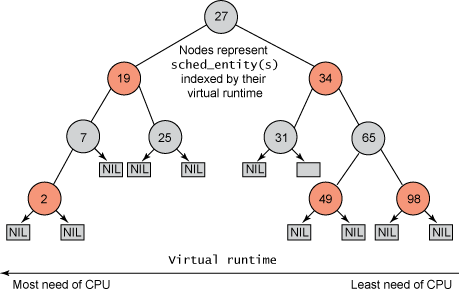
\includegraphics[width=3.0in]{figure1.png}
\caption{\og CFS \fg ~ arbre rouge-noir sur le temps d'exécution - image issue de IBM \citep{jones2009inside}.}
\label{fig1}
\end{center}
\end{figure}

Si le processus passe beaucoup de temps à dormir, alors son temps passé est faible et recevra donc automatiquement une augmentation en priorité lorsqu'il en aura besoin. Par conséquent, de telles tâches n'obtiennent pas moins de temps processeur que celles qui fonctionnent continuellement \citep{Wong:2008:TAF:1400097.1400102}.

L'idée du CFS est dérivée du \textit{Weighted Fair Queueing} utilisé par les ordonnanceurs réseau qui s'occupent de la distribution des paquets de données \citep{Demers:1989:ASF:75247.75248}. La conversion vers la gestion des processus s'est effectuée au travers du \textit{stride scheduling}. En effet, celui-ci propose un mécanisme d'ordonnancement des ressources déterministes qui calcule un intervalle de temps ou \textit{stride} pendant lequel chaque client attend et qui est également proportionnel à sa propre consommation des ressources \citep{Waldspurger:1995:LSS:888601}.

Le CFS a reçu un patch en novembre 2010 (2.6.38) pour le rendre plus équitable sur les stations de travail et bureaux, appuyé par des tests de performances effectués plus tôt \citep{7280991}. Sur une idée de Torvalds et les travaux de Galbraith, il regroupe des \textit{threads} afin de mieux servir les applications multi-tâches \citep{Wong:2008:TAF:1400097.1400102}. Depuis, il semble être plus équitable et plus efficace que l'ordonnanceur $O(1)$ \citep{4631872}.

Après la sortie de cet ordonnanceur, il n'y a plus eu de grandes modifications dans le système d'ordonnancement, seulement des corrections et des ajustements.

\subsection{BFS:}

Le CFS a eu un petit frère également développé par Con Kolivas et dénommé \textit{Brain Fuck Scheduler} parce que, selon les mots de son créateur, il brise les codes actuels de design en matière de mise à l'échelle. Il a pour but d'être le concurrent du CFS sur des modèles multicœurs \citep{PATCHBFS}. Il n'est pas un ordonnanceur officiel, en ce sens qu'il n'est pas incorporé au noyau Linux \citep{opac-b1133216}. Malgré le fait qu'il offre des meilleurs temps de réaction que le CFS et est parfois plus rapide que celui-ci pour accomplir certaines tâches, il a dû mal à passer à l'échelle ou à fonctionner sur des systèmes à accès mémoire non-uniforme (NUMA). Il est surtout destiné à un usage de type bureautique sur les architectures actuelles \citep{CFSVSBFS}.

\section{Les types temps réel}

Linux n'est pas un système d'exploitation conçu pour les tâches temps réelles mais propose quand même certaines notions notamment au niveau des ordonnanceurs qualifiés de \textit{Soft real-time} où une tolérance est permise au niveau des échéances. L'idée du temps réel est de diviser le travail en petites tâches prédictibles et connues à l'avance afin de pouvoir quantifier le temps nécessaire à leur réalisation et donc permettre une meilleure prédictabilité. Le but des ordonnanceurs est dès lors de s'assurer que chaque processus puisse respecter ses propres limites temporelles \citep{stankovic2012deadline}.

Il y a également une distinction effectuée entre les tâches dites périodiques et apériodiques qui représentent respectivement des actions étant réalisées de manière récurrente et celles surgissant de manière non prédictible. Dès lors, on peut se demander si les objectifs peuvent être respectés et on établit une condition de faisabilité afin de prouver l'efficacité de cet ordonnanceur \citep{128746}. Énormément de travaux ont été effectués sur ce sujet \citep{Sha:2004:RTS:1028913.1028959}.

\subsection{Début FIFO et RR}

Linux se conforme globalement à la norme \textit{POSIX}, nottament avec ces politiques temps réel à priorité fixe (SCHED\_FIFO \& SCHED\_RR). Ces algorithmes sont relativement efficaces lorsqu'il y a peu de tâches mais ont du mal à passer à l'échelle. Le FIFO minimise le temps de réponse de l'ensemble des tâches et toutes les tâches partagent le même temps maximal. Il n'est pas optimal pour des tâches ayant des échéances différentes et peut créer des inversions de priorités \citep{Klein:1993:PHR:174003}. Le Round Robin est théoriquement plus équitable mais il risque d'être déséquilibré si les tâches ont des délais différents, de plus il n'est pas optimal même si des améliorations ont été proposées \citep{Shreedhar:1995:EFQ:217391.217453}.

Les premières grandes avancées sur cette problématique dans le noyau Linux débutèrent avec la version 2.4.18, et ses algorithmes \textit{Constant Bandwidth Server} \citep{Abeni:1998:IMA:827270.829047} et \textit{Greedy Reclamation of Unused Bandwidth} \citep{Lipari:2000:GRU:1947412.1947445} qui réclament les ressources non utilisées du processeur. Le problème à cette époque était le manque de support multicœur et la difficulté de porter vers des versions différentes du noyau. Il fallait également se défaire du \textit{Big Kernel Lock}. Notons, que des politiques spéciales \textit{SCHED\_SOFTRR} et \textit{SCHED\_ISO} sont apparues et permettent aux utilisateurs privilégiés de faire tourner les tâches en temps réel jusqu'à usage complet du processeur \citep{scordino2006linux}.

\subsection{Earliest deadline first}

Le \textit{SCHED\_DEADLINE} apparaît officiellement avec la version 3.14 du noyau. Il est issu d'un travail de plusieurs années et est davantage connu comme une implémentation du Earliest Deadline First \citep{faggioli2009edf}. Il vise à remplacer les poliques \textit{RR} et \textit{FIFO} qui ne correspondent pas tout à fait aux attentes des tâches temps réelles \citep{buttazzo2011hard}. L'idée sous-jacente à cet algorithme est de travailler avec une file à priorité ordonnée par rapport au temps restant avant l'échéance. Des résultats théoriques ayant été obtenus auparavant suite aux travaux de Liu et Layland \citep{liu1973scheduling}.

\newcommand{\pluseq}{\mathrel{+}=}

L'algorithme en lui-même:
On appelle \textit{$q_i$} le temps restant d'éxécution (le temps processeur que la tâche peut utilisée avec sa période \textit{$T_i$} et \textit{$Q_i$} sa fin), et \textit{$d_i$} une échéance qui permet d'assigner dynamiquement la priorité \citep{LelliEDFLinux}.

Au début, \textit{$q_i$} et \textit{$d_i$} valent 0.
Quand une tâche se réveille à l'instant $t$, l'ordonnanceur regarde si son $d_i$ est toujours valable (soit si $q_i < (d_i - t) * Q_i/ T_i$), sinon il redéfinit $d_i = t + T_i$ et $Q_i \pluseq q_i$. Quand une tâche s'exécute, son $q_i$ est diminué du temps effectué. Si $q_i$ arrive à 0, la tâche est suspendue et ne peut être sélectionnée par l'ordonnanceur pour exécution (parce qu'il ne respecterait pas alors le $Q_i$ sur une période $T_i$). La tâche est reprise seulement au temps $t = d_i$, son $q_i$ sera alors égale à $Q_i$ et son échéance postposée à $d_i \pluseq T_i$.

Cependant ce genre d'algorithmes est généralement conçu pour des processeurs monocœurs. Lorsque plusieurs processus peuvent être exécutés en même temps, on distingue deux cas d'ordonnanceur \citep{faggioli2009implementation}: les globaux et les partitionnés (et des hybrides). Dans le global, toutes les tâches sont fournies à la même structure de donnée qui les distribue sur les différents cœurs alors que dans le partionné, différentes listes sont maintenues pour chaque cœur. Ils ont chacun leurs avantages et inconvénients et il y a beaucoup de littérature sur ce sujet \citep{bastoni2010empirical, lelli2012experimental}.
En l'occurrence, Linux utilise une file de tâches distribuée, c'est-à-dire que chaque cœur à sa propre file mais que des tâches peuvent être transférées de l'une vers l'autre.

L'un des plus gros problèmes du temps réel est lié aux ressources partagées \citep{buttazzo2011hard}. En effet, les sections critiques peuvent entraîner une grande surcharge de travail, ou des risques d'inversions de priorité. On améliore généralement ces algorithmes avec ce qui s'appelle \textit{deadline inheritance over shared resources} ou \textit{DFP} \citep{jansen2003lightweight}. Il existe également des \textit{serveurs} qui visent à améliorer l'utilisation sur les différents cœurs en utilisant les ressources au maximum, en équilibrant au mieux la charge. Notamment, le \textit{Bandwidth Inheritance algorithm}, extension du \textit{Constant Bandwidth Server} \citep{Abeni:1998:IMA:827270.829047} intégré au noyau Linux en même temps que le \textit{EDF}. Ou encore un de ses enfants, le \textit{Greedy Reclamation of Unused Bandwidth} \citep{Lipari:2000:GRU:1947412.1947445}. Citons également, le \textit{Barbershop Load
Distribution algorithm} de Rakib Mullick qui tendrait à mieux répartir les tâches en fonction de la charge présente sur les cœurs \citep{BarbershopLoadDistribution}.

\section{Discussion}

Nous avons vu la situation chez Linux mais qu'en est-il pour d'autres grands systèmes d'exploitation ? Ont-ils opté pour les mêmes choix d'ordonnancement ? Si non, quelles en sont les raisons ?

\subsection{Microsoft}

Chez Microsoft, depuis Windows NT, un ordonnanceur avec plusieurs files à priorités est employé. Il correspond plus ou moins à l'idée du $O(n) / O(1)$ mais avec 32 priorités dont 16 concernent les opérations relatives au \textit{soft real-time} et la priorité 0 au système de nettoyage des pages mémoires inutilisées \citep{jones1999cpu}. Nottons que cet ordonnanceur n'effectue pas de distinctions entre les tâches d'un même programme et les programmes en eux-mêmes. Si un processus A possède 10 \textit{threads} et B en détient 2, chaque \textit{thread} recevra théoriquement un douzième du temps imparti pour l'ensemble des tâches. Windows propose plus de status différents possibles pour les tâches comparativement à Linux et que depuis Vista, le registre qui comptabilise le nombre de cycles effectués par un programme est employé \citep{Russinovich:2009:WII:1717352}. Il existe également, depuis Windows 7, la possibilité d'utiliser son propre ordonnanceur pour ses tâches appelé \textit{User-Mode Scheduling} \citep{UMS}.

\subsection{Apple}

Chez Apple, depuis Mac OS X, la situation est analogue à celle de Linux, suite à leur certification à la norme \textit{POSIX}. À la différence près qu'un ordonnanceur à base de files à priorités est employé par défaut, sorte de $O(1)$. La borne pour les priorités associées à chaque tâche est très élevée et permet donc plus de finesse. Il existe quatre subdivisions dans les priorités: les normales, les élevées, les noyaux et les temps réels \citep{singh2006mac}.

\subsection{BSD}

Chez FreeBSD, depuis la version 7.1, un ordonnanceur dénomé \textit{ULE} est employé. Il a remplacé un \textit{Round-robin} qui se faisait vieillissant et qui ne supportait pas les nouveautés matérielles (SMT / SMP). Le nouveau, \textit{ULE}, emploie trois files de tâches exécutables: deux sont réservées à toutes les tâches courantes et une à ceux en attente. À la différence de bon nombre d'ordonnanceurs, il réagit au travers d'événements et non par le biais de quantums de temps \citep{roberson2003ule}. L'équité et l'absence de famine sont assurées par le fait que les files sont parcourues entièrement en fonction de leur priorité. Cette priorité est calculée en fonction du temps réellement employé dans l'intervalle accordé. Ce système se rapproche des files à priorités mais avec des différences notables \citep{mckusick2014design}.

\subsection{Analyse}

Nous voyons que, parmi ces exemples, les ordonnanceurs employés par ces systèmes d'exploitation sont basés sur les modèles des files à priorités et non celui d'un arbre. On peut donc se demander ce qui justifie une telle différence. Linux a abandonné les files au profit du CFS basé davantage sur sur l'équité et sur le modèle théorique du \textit{stride scheduling}. Si on se base sur les résultats des articles de Wong, Tan, Kumari et Lam \citep{4631872, Wong:2008:TAF:1400097.1400102}, le CFS permet de faire diminuer la variance dans le temps mis pour accomplir une tâche. Le $O(1)$ donne un résultat plus étendu sur la plage des temps, il offre donc une moins bonne équité. La différence d'interactivité n'est presque pas perceptible mais donne un très léger avantage au $O(1)$. Wang, Chen, Jiang et Li \citep{5279631} et Pabla \citep{Pabla:2009:CFS:1594371.1594375} arrivent à peu près aux mêmes conclusions.

Si les performances de ce système sont analogues en permettant une meilleure équité, qu'en est-il de sa mise à l'échelle ? Si on se réfère à l'article Li, Baumberger et Hahn \citep{li2009efficient} qui propose une comparaison de différents type d'ordonnancement, le CFS est analogue au WFQ par design et possède donc une complexité en $O(log N)$ avec une latence positive constante mais dont la latence négative est borné par $O(n)$ \citep{234856}. A contrario, les ordonnanceurs basés sur des files à priorités possèdent une complexité en $O(1)$, mais ont une plus faible équité avec une latence bornée par $O(n)$ en général. Seulement, si les poids des tâches sont bornés par une constante, ce qui est une hypothèse qui peut être appliquée à la pratique, alors la latence tant positive que négative peut être bornée par une constante \citep{Shreedhar:1995:EFQ:217391.217453}.

Ces résultats théoriques peuvent être altérés par des détails d'implémentation qui les rendraient plus lents ou, au contraire, plus rapides. Seulement, on doute que des géants tels que Microsoft optent pour un système moins performant. Il serait intéressant de faire une comparaison des deux familles. Signalons qu'il y a encore des problèmes de performances dans les dernières versions du noyau Linux, nottament vis-à-vis de NUMA \citep{lozi2016linux, blagodurov2010case} qui peuvent être expliqués par la difficulté d'étudier la régression chez les ordonnanceurs \citep{chen2007keeping} et que la nécessité de développer des outils de tests approfondis est plus que cruciale afin de s'assurer de la justesse de ceux-ci \citep{erickson2010effective}.

\section{Conclusion}

Implémenter un ordonnanceur n'est pas une tâche aisée, et le rendre correct d'un point de vue formel est encore plus difficile. Nous avons vu que la route fut longue pour arriver à l'état actuel, qui est encore loin d'être parfait. Des concepts pourtant simples peuvent se retrouver mis à mal face à la complexité et la diversité des matériels disponibles, outre les détails d'implémentation. Le problème, même si bon nombres de résultats théoriques ont déjà été obtenus, demeure ouvert et il faut rester réactif face aux nouveautés matérielles apportées par les avancées technologiques.

\footnotesize
\bibliographystyle{apalike}
\bibliography{bibliography}

\end{document}
